% Generated from both complete registered stages by make_query_assets.py.
% Figure data retain every repeat; independent audit findings are not inferred here.
\begin{figure*}[t]
\centering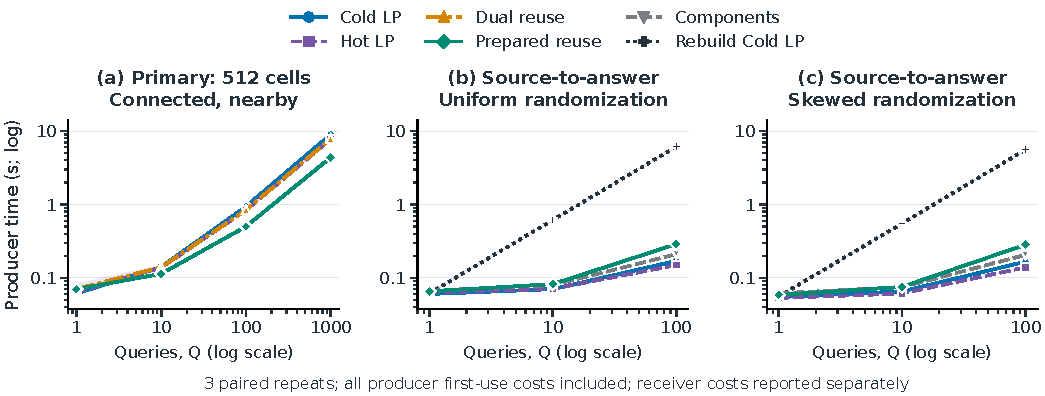
\includegraphics[width=\textwidth]{figures/query_cumulative_v2.pdf}
\caption{Cumulative producer time, including first-use costs. Lines show medians over three paired repetitions; shaded bands show the minimum and maximum, not confidence intervals. Both axes use logarithmic scales and time is in seconds. In (b)--(c), all plans except Rebuild Cold LP materialize once. Only measured prefixes are plotted: the source-to-answer runs stop at 100 queries. Consumer proof checking is reported separately in Table~\ref{tab:query-consumer}.}
\label{fig:query-cumulative}
\end{figure*}

\textbf{Registered timing result.} Both execution stages completed: 54 controlled conditions with seven plans and six source-to-answer conditions with five plans. For the registered 512-cell connected nearby-query workload, Prepared reuse takes a median 4.37\,s for 1,000 queries, against 7.76\,s for Hot LP. The three paired time ratios are 0.5141, 0.5640, 0.5751 (median 0.5640). All three meet the registered $\leq0.8$ timing condition. Figure~\ref{fig:query-cumulative} retains the first query, initialization, all later misses, and response serialization. Three timings support a descriptive comparison, not a significance test.

\textbf{Workload boundary.} At $Q=100$, Prepared reuse is no slower than Hot LP in 9 of 18 cells. The largest median paired ratio is 10.704, for 512 cells with mixed structure and unrelated objectives. The artifact retains the full grid, all seven-plan timings and every repeat; the 2,048-cell grid stops at its registered 100-query cap. These are execution fixtures, not coverage or policy-utility experiments.

\textbf{Source-to-answer cost.} With uniform randomization, 100 measured queries take 0.289\,s for materialized Prepared reuse, 0.15\,s for materialized Hot LP and 6.12\,s for rebuilding; the median paired Prepared/Hot ratio is 1.930. With skewed randomization, 100 measured queries take 0.284\,s for materialized Prepared reuse, 0.14\,s for materialized Hot LP and 5.56\,s for rebuilding; the median paired Prepared/Hot ratio is 2.031. These totals include reading, validating and aggregating five million encoded events, source intervals, feasible-view construction, execution and response serialization. The comparison with materialized Hot LP isolates the remaining execution benefit after shared input work is retained.

\textbf{Reuse and bound tightness.} Prepared reuse serves 18,873/38,400 queries from saved duals; the remaining 19,527 comprise 19,527 solver fallbacks, 0 box shortcuts and 0 refusals. There are 0 certification disagreements with Hot LP. Across finite matched answers, Prepared-minus-Hot lower bounds range from $-0.008128$ to $1.821\times10^{-17}$ in success-probability units. A hit proves enough for the threshold, not necessarily the tightest bound. Across all plans, recorded replay verifies 267,600 proofs with 0 no-bound responses; independent audit is a separate check.

\begin{table*}[t]
\centering
\caption{Measured producer and consumer costs in seconds. Each entry is a three-repeat median. Joint costs add producer time, fresh checker initialization, JSON decoding and proof verification within each repeat before taking the median; Joint/Hot is the median paired joint-cost ratio. Thus the displayed component medians need not sum exactly to the joint median. Compression, compressed-file reading/decompression and unmeasured network transfer are excluded from the joint total.}
\label{tab:query-consumer}\begingroup\fontsize{8}{9.4}\selectfont\setlength{\tabcolsep}{3.5pt}
\begin{tabular*}{\textwidth}{@{\extracolsep{\fill}}llrrrrrr@{}}
\toprule
Workload & Plan & Producer & Checker init. & JSON decode & Verify & Joint & Joint / Hot\\
\midrule
Primary, 1,000 queries & Hot LP & 7.76 & 0.00924 & 0.29 & 8.24 & 16.2 & 1.000\\
 & Prepared reuse & 4.37 & 0.00932 & 0.286 & 10.1 & 14.7 & 0.906\\
Uniform, 100 queries & Hot LP & 0.15 & 0.00114 & 0.00466 & 0.0833 & 0.238 & 1.000\\
 & Prepared reuse & 0.289 & 0.00104 & 0.00445 & 0.0828 & 0.377 & 1.580\\
Skew, 100 queries & Hot LP & 0.14 & 0.00116 & 0.00458 & 0.0832 & 0.229 & 1.000\\
 & Prepared reuse & 0.284 & 0.00107 & 0.00448 & 0.0831 & 0.372 & 1.619\\
\bottomrule
\end{tabular*}
\endgroup

\end{table*}

\textbf{Cost beyond the producer.} Table~\ref{tab:query-consumer} charges the receiving checker explicitly. Adding its measured work changes the Prepared/Hot comparison to 0.906 for the primary engine workload, 1.580 for uniform source-to-answer and 1.619 for skewed source-to-answer. These joint ratios prevent a producer-only result from concealing work moved to a consumer. Compressed-proof writing is recorded separately; these are not full deployment-latency measurements. The maximum saved-dual bank contains 16 entries. The largest final prepared-term Python payload is 343.9\,KiB, excluding shared view endpoints. This payload is not native solver RSS; the process-wide high-water mark is not isolated by plan.
